\documentclass{article}%
\usepackage[T1]{fontenc}%
\usepackage[utf8]{inputenc}%
\usepackage{lmodern}%
\usepackage{textcomp}%
\usepackage{lastpage}%
\usepackage[head=40pt,margin=0.5in,bottom=0.6in]{geometry}%
\usepackage{graphicx}%
%
\title{\textbf{Falleció el afamado narrador deportivo Tury Agüero}}%
\author{Diario El Universal}%
\date{03/03/2019}%
%
\begin{document}%
\normalsize%
\maketitle%
\textbf{URL: }%
http://www.eluniversal.com/sucesos/34710/fallecio{-}el{-}recordado{-}narrador{-}deportivo{-}tury{-}agero\newline%
%
\textbf{Periodico: }%
EU, %
ID: %
34710, %
Seccion: %
sucesos\newline%
%
\textbf{Palabras Claves: }%
NO\_TIENE\newline%
%
\textbf{Derecho: }%
2.1%
, Otros Derechos: %
\newline%
%
\textbf{\textit{Durante los años 70 y 80 fue una de las referencias en la locución deportiva en Venezuela, destacando en fútbol, boxeo y todo lo relacionado al automovilismo con su recordado programa "A Toda Máquina"}}%
\newline%
\newline%
%
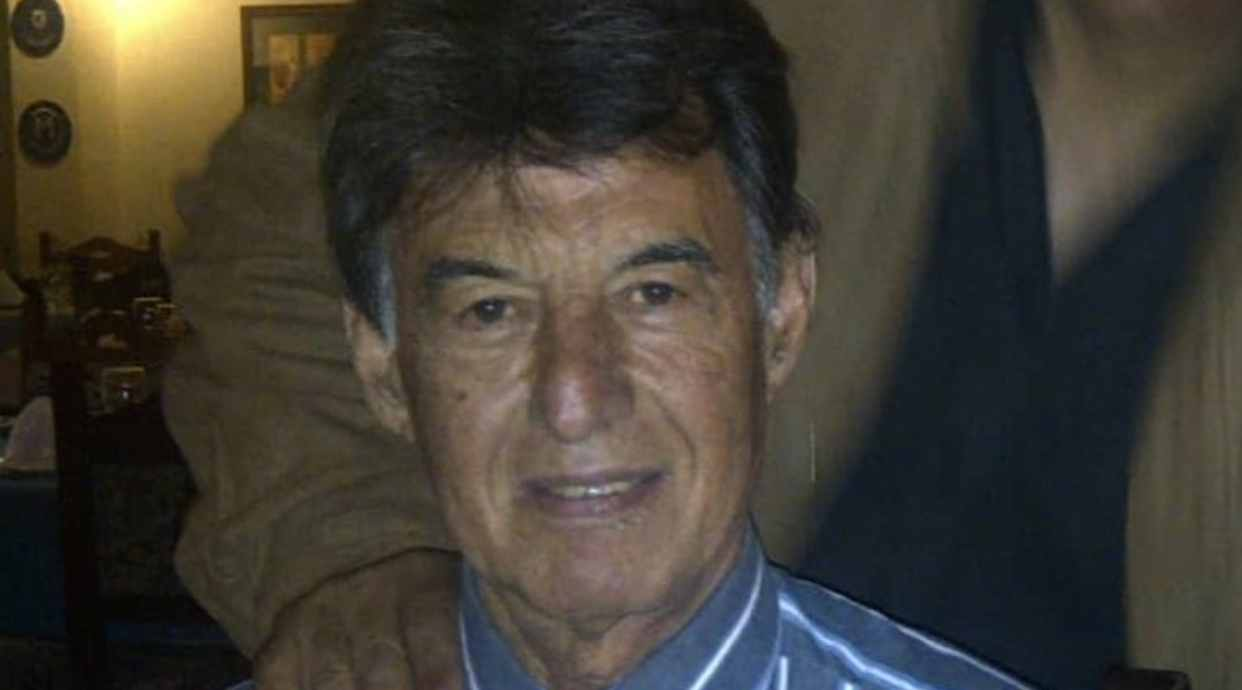
\includegraphics[width=300px]{EU_34710.jpg}%
\newline%
%
Caracas.{-} Este domingo se pudo conocer a través de las redes sociales del fallecimiento del gran narrador deportivo, Tury Agüero, quien era una de los referentes del área deportiva de Venezolana de Televisión durante las décadas del 70, 80 e inicio de los 90.%
\newline%
%
A pesar de brillar en deportes tan distintos como el fútbol y el boxeo, Agüero es recordado con cariño especialmente por los amantes del automovilismo gracias a su programa "A Toda Máquina", que cubría este apasionante mundo de los motores.%
\newline%
%
Su muerte llena de tristeza a la comunicación venezolana en general; sin embargo, recibió muchas muestras de aprecio en la red social Twitter por colegas que lamentaron su sorpresiva partida.%
\newline%
%
Aún se desconoce el motivo de su deceso por lo que habrá que esperar un pronunciamiento al respecto por parte de sus allegados.%
\newline%
%
\end{document}